\documentclass[11pt]{article}

\usepackage[review]{acl}

\usepackage{times}
\usepackage{latexsym}
\usepackage[T1]{fontenc}
\usepackage[utf8]{inputenc}
\usepackage{microtype}
\usepackage{inconsolata}
\usepackage{graphicx}
\usepackage{amsmath,amssymb}
\usepackage{booktabs}
\usepackage{multirow}
\usepackage{tabularx}
\usepackage{enumitem}
\usepackage{xcolor}

\newcommand{\bench}{\textsc{ForceBench}}
\newcommand{\tbd}{\textcolor{gray}{--}}

\title{\bench{}: Unifying Cross-Embodiment Tactile Sensing via Canonical Hand-Surface Retargeting and Frozen Representation Probing}

\author{Anonymous ACL Submission}

\begin{document}
\maketitle

\begin{abstract}
Tactile sensing is essential for contact-rich robotic manipulation, yet tactile data remains fragmented across heterogeneous sensor modalities, resolutions, and robot embodiments---ranging from multi-fingered dexterous hands to two-finger parallel grippers.
Moreover, existing tactile representation encoders are typically evaluated by their own native reconstruction losses or task-specific fine-tuning, obscuring how much contact geometry, intensity trend, and dynamic information is actually preserved and linearly or compactly readable from frozen latent representations.
In this work, we present \bench{}, a unified cross-embodiment tactile data pipeline and frozen representation benchmark.
First, we introduce two complementary retargeting pipelines---inverse vector retargeting with distal-phalanx surface projection for articulated dexterous hands, and fixed surface correspondence (extended via a general \texttt{StandardPad} trend mode) for parallel grippers---that map heterogeneous tactile streams onto a canonical $128\times 128$ MANO UV hand-surface atlas while strictly separating observed contact trends from sensor validity masks.
Second, we curate a unified multi-source dataset spanning six dexterous-hand and visuo-tactile gripper corpora under a read-only, fixed-scale data contract without per-frame auto-normalization.
Third, we establish a three-level evaluation hierarchy (L0 information retention, L1 frozen readability of contact proxies, verified physical forces, and temporal dynamics, and L2 cross-source, cross-embodiment, and perturbation generalization) under a fair frozen-encoder probing protocol, and benchmark a suite of self-trained reconstruction (\texttt{zero}) and latent-prediction (\texttt{JEPA}) encoders alongside non-learned and external baselines.
\end{abstract}

\section{Introduction}
\label{sec:intro}

Rich tactile feedback is indispensable for dexterous manipulation, enabling agents to perceive contact localization, load distribution, and incipient slip that vision alone cannot reliably resolve.
Despite rapid progress in tactile hardware and self-supervised tactile encoders \citep{higuera2024sparsh,feng2025anytouch}, building general-purpose tactile representations remains bottlenecked by two structural barriers.

First, \textbf{cross-embodiment and cross-sensor heterogeneity} fractures tactile datasets into incompatible silos.
Articulated dexterous hands (e.g., 22-DoF multi-fingered hands with fingertip deformation arrays) and two-finger parallel grippers (e.g., vision-based tactile sensors outputting RGB images or depth reconstructions) differ in kinematics, sensor geometry, physical quantity, and spatial coverage.
Directly pooling raw tactile signals across embodiments is infeasible without a shared anatomical coordinate system, while naive per-frame normalization destroys absolute contact-intensity trends and conflates unobserved sensor regions with zero contact.

Second, \textbf{evaluation protocols for tactile encoders lack comparability and diagnostic rigor}.
Prior work frequently compares encoders using their own training objectives, native decoders of unequal capacity, or end-to-end downstream fine-tuning.
Such protocols cannot answer three fundamental questions about a \emph{frozen} tactile representation:
(1) \emph{Information retention}: how accurately does the latent preserve contact location, spatial distribution, and intensity trends?
(2) \emph{Frozen readability}: how easily can contact-related and physical quantities be decoded by low-capacity, standardized probes?
(3) \emph{Generalization}: does this readability hold across data sources, embodiments, physical quantities, and input perturbations?

To address these challenges, we introduce \bench{}, a unified cross-embodiment tactile retargeting framework, curated canonical dataset, and frozen representation benchmark.
Crucially, we enforce a strict physical terminology and data contract: uncalibrated UV gray-level signals represent \emph{tactile intensity / contact proxy trends} rather than calibrated Newton forces, and physical units (N or N$\cdot$m) are reported exclusively when independent external wrench labels pass unit, coordinate-frame, and temporal alignment verification.

Our contributions are threefold:
\begin{itemize}[leftmargin=*,nosep]
    \item \textbf{Dual-Route Cross-Embodiment Retargeting:} We develop two complementary pipelines mapping heterogeneous tactile embodiments onto a canonical $128\times 128$ MANO UV atlas \citep{romero2017embodied}: (i) an articulated dexterous-hand route combining inverse vector retargeting, Umeyama alignment, and distal-phalanx KD-tree surface projection; and (ii) a parallel-gripper route combining automated no-contact reference selection, depth reconstruction, and static surface correspondence, alongside a general \texttt{StandardPad} trend mode for arbitrary gripper tactile arrays.
    \item \textbf{Unified Multi-Source Canonical Dataset:} Applying these pipelines under a strict fixed-scale, read-only data contract, we unify six diverse manipulation corpora---five Sharpa dexterous-hand sources and one visuo-tactile gripper source---into a standardized bimanual UV video format ($128\times 256$, 30~FPS) with explicit separation of contact trends and sensor validity masks.
    \item \textbf{Frozen Representation Benchmark and Encoder Validation:} We construct \bench{} with a hierarchical L0--L2 task suite, standardized low-capacity probes (projected readout, $k$-NN, and attentive readout), episode-level splits, and rigorous statistical testing. Using our unified data, we train and systematically evaluate a controlled family of CNN and ViT tactile encoders under pixel-reconstruction (\texttt{force\_encoder\_zero}) and latent-prediction (\texttt{force\_encoder\_jepa}) objectives against non-learned and external baselines.
\end{itemize}

\section{Related Work}
\label{sec:related}

\subsection{Tactile Representation Learning and Cross-Embodiment Retargeting}
Self-supervised representation learning has emerged as a promising paradigm for tactile sensing, adapting masked autoencoding, contrastive learning, and joint-embedding predictive architectures (JEPA) \citep{assran2023self,bardes2024revisiting} to visuo-tactile images and taxel arrays.
\citet{higuera2024sparsh} pre-train visuo-tactile encoders via MAE, DINO, and JEPA objectives on RGB elastomer images, while \citet{feng2025anytouch} learn static-dynamic representations across multiple visuo-tactile sensors using sensor-specific tokens.
However, these approaches predominantly operate in sensor-native image or taxel spaces, making cross-embodiment transfer between articulated dexterous hands and parallel grippers difficult.
On the geometric side, parametric human hand models such as MANO \citep{romero2017embodied} provide a canonical surface parameterization widely used for kinematic hand retargeting.
Unlike prior kinematic-only retargeting pipelines, our dual-route framework maps \emph{both} articulated hand kinematics with fingertip deformation arrays and static parallel-gripper tactile pads onto the same canonical MANO UV atlas under fixed, non-adaptive intensity scaling.

\subsection{Tactile and Embodied Manipulation Benchmarks}
Existing tactile evaluation suites largely focus on single-sensor classification, material recognition, or end-to-end policy success in simulation.
While informative for specific hardware, such benchmarks conflate encoder representation quality with downstream policy capacity, decoder architecture, or sensor-specific visual artifacts.
Table~\ref{tab:benchmark_comparison} contrasts \bench{} with representative tactile representation and manipulation benchmarks across embodiment coverage, canonicalization, validity masking, and evaluation protocol.
\bench{} is uniquely designed to isolate \emph{frozen} encoder latent quality across embodiments via unified small-decoder reconstruction (L0), decoupled proxy/physical/temporal probing (L1), and controlled cross-domain generalization (L2).

\begin{table*}[t]
\centering
\small
\setlength{\tabcolsep}{4.5pt}
\begin{tabular}{lccccccc}
\toprule
\textbf{Benchmark / Suite} & \textbf{Canonical} & \textbf{Dexterous +} & \textbf{Validity} & \textbf{Frozen} & \textbf{Unified} & \textbf{Temporal} & \textbf{Cross-Emb.} \\
 & \textbf{Surface} & \textbf{Gripper} & \textbf{Mask} & \textbf{Probes} & \textbf{Decoder} & \textbf{Dynamics} & \textbf{Transfer} \\
\midrule
Sparsh Suite \citep{higuera2024sparsh} & -- & Gripper only & -- & \checkmark & -- & Partial & -- \\
AnyTouch Eval \citep{feng2025anytouch} & -- & Gripper only & -- & \checkmark & -- & \checkmark & -- \\
Sensor-Native Recon. Baselines & -- & Single & -- & -- & -- & -- & -- \\
\midrule
\textbf{\bench{} (Ours)} & \textbf{MANO UV} & \textbf{\checkmark} & \textbf{\checkmark} & \textbf{\checkmark} & \textbf{\checkmark} & \textbf{\checkmark} & \textbf{\checkmark} \\
\bottomrule
\end{tabular}
\caption{Comparison of \bench{} with existing tactile representation evaluation protocols. \bench{} unifies articulated dexterous hands and parallel grippers onto a canonical MANO UV atlas with explicit observation validity masks and standardized frozen-encoder probing.}
\label{tab:benchmark_comparison}
\end{table*}

\section{Cross-Embodiment Tactile Unification}
\label{sec:retarget_data}

\subsection{Canonical Surface and Data Contract}
\label{sec:data_contract}
To unify heterogeneous robot morphologies without discarding spatial contact topology, we project all tactile streams onto the official $128\times 128$ MANO UV atlas \citep{romero2017embodied} per hand and horizontally concatenate bimanual recordings into standardized $128\times 256$ streams at 30~FPS.

To guarantee physical rigor and prevent silent evaluation artifacts, every source adheres to a three-part \textbf{data contract}:
\begin{enumerate}[leftmargin=*,nosep]
    \item \textbf{Contact Proxy vs.\ Physical Force:} Uncalibrated UV intensities encode sensor-specific contact proxies---such as fingertip deformation luminance (Sharpa) or elastomer depth proxies (TacVerse)---rather than calibrated Newton forces. Unified UV geometry does not imply unified force semantics across heterogeneous sensors; physical units (N or N$\cdot$m) are reported exclusively when independent external wrench labels pass unit, coordinate-frame, and temporal alignment verification.
    \item \textbf{Observed-Zero vs.\ Unknown:} Each texel separates its contact value from an explicit observation validity indicator, distinguishing the \emph{MANO UV foreground mask} (hand surface vs.\ background) from the \emph{sensor observation mask} (instrumented pads vs.\ uninstrumented fingers or palm). Unobserved regions---which also render dark in UV maps---are excluded from statistics rather than conflated with zero contact.
    \item \textbf{Fixed Global Scaling:} Source streams remain read-only and are mapped through fixed global or training-frozen scalers. Per-frame auto-normalization is strictly prohibited so that relative contact-load trends remain comparable across time.
\end{enumerate}

\subsection{Dual-Route Retargeting}
\label{sec:retarget_pipelines}
Because articulated dexterous hands and two-finger parallel grippers differ in kinematics and sensor mounting, we formulate both pipelines under the same four-stage abstraction---(1)~\emph{Input \& Preprocessing}, (2)~\emph{MANO Alignment}, (3)~\emph{Surface Projection}, and (4)~\emph{Fixed-Scale UV Export}---specializing only the embodiment-dependent alignment and projection steps (Figure~\ref{fig:retarget_pipeline}; implementation constants in Appendix~\ref{app:retarget}).

\begin{figure*}[t]
    \centering
    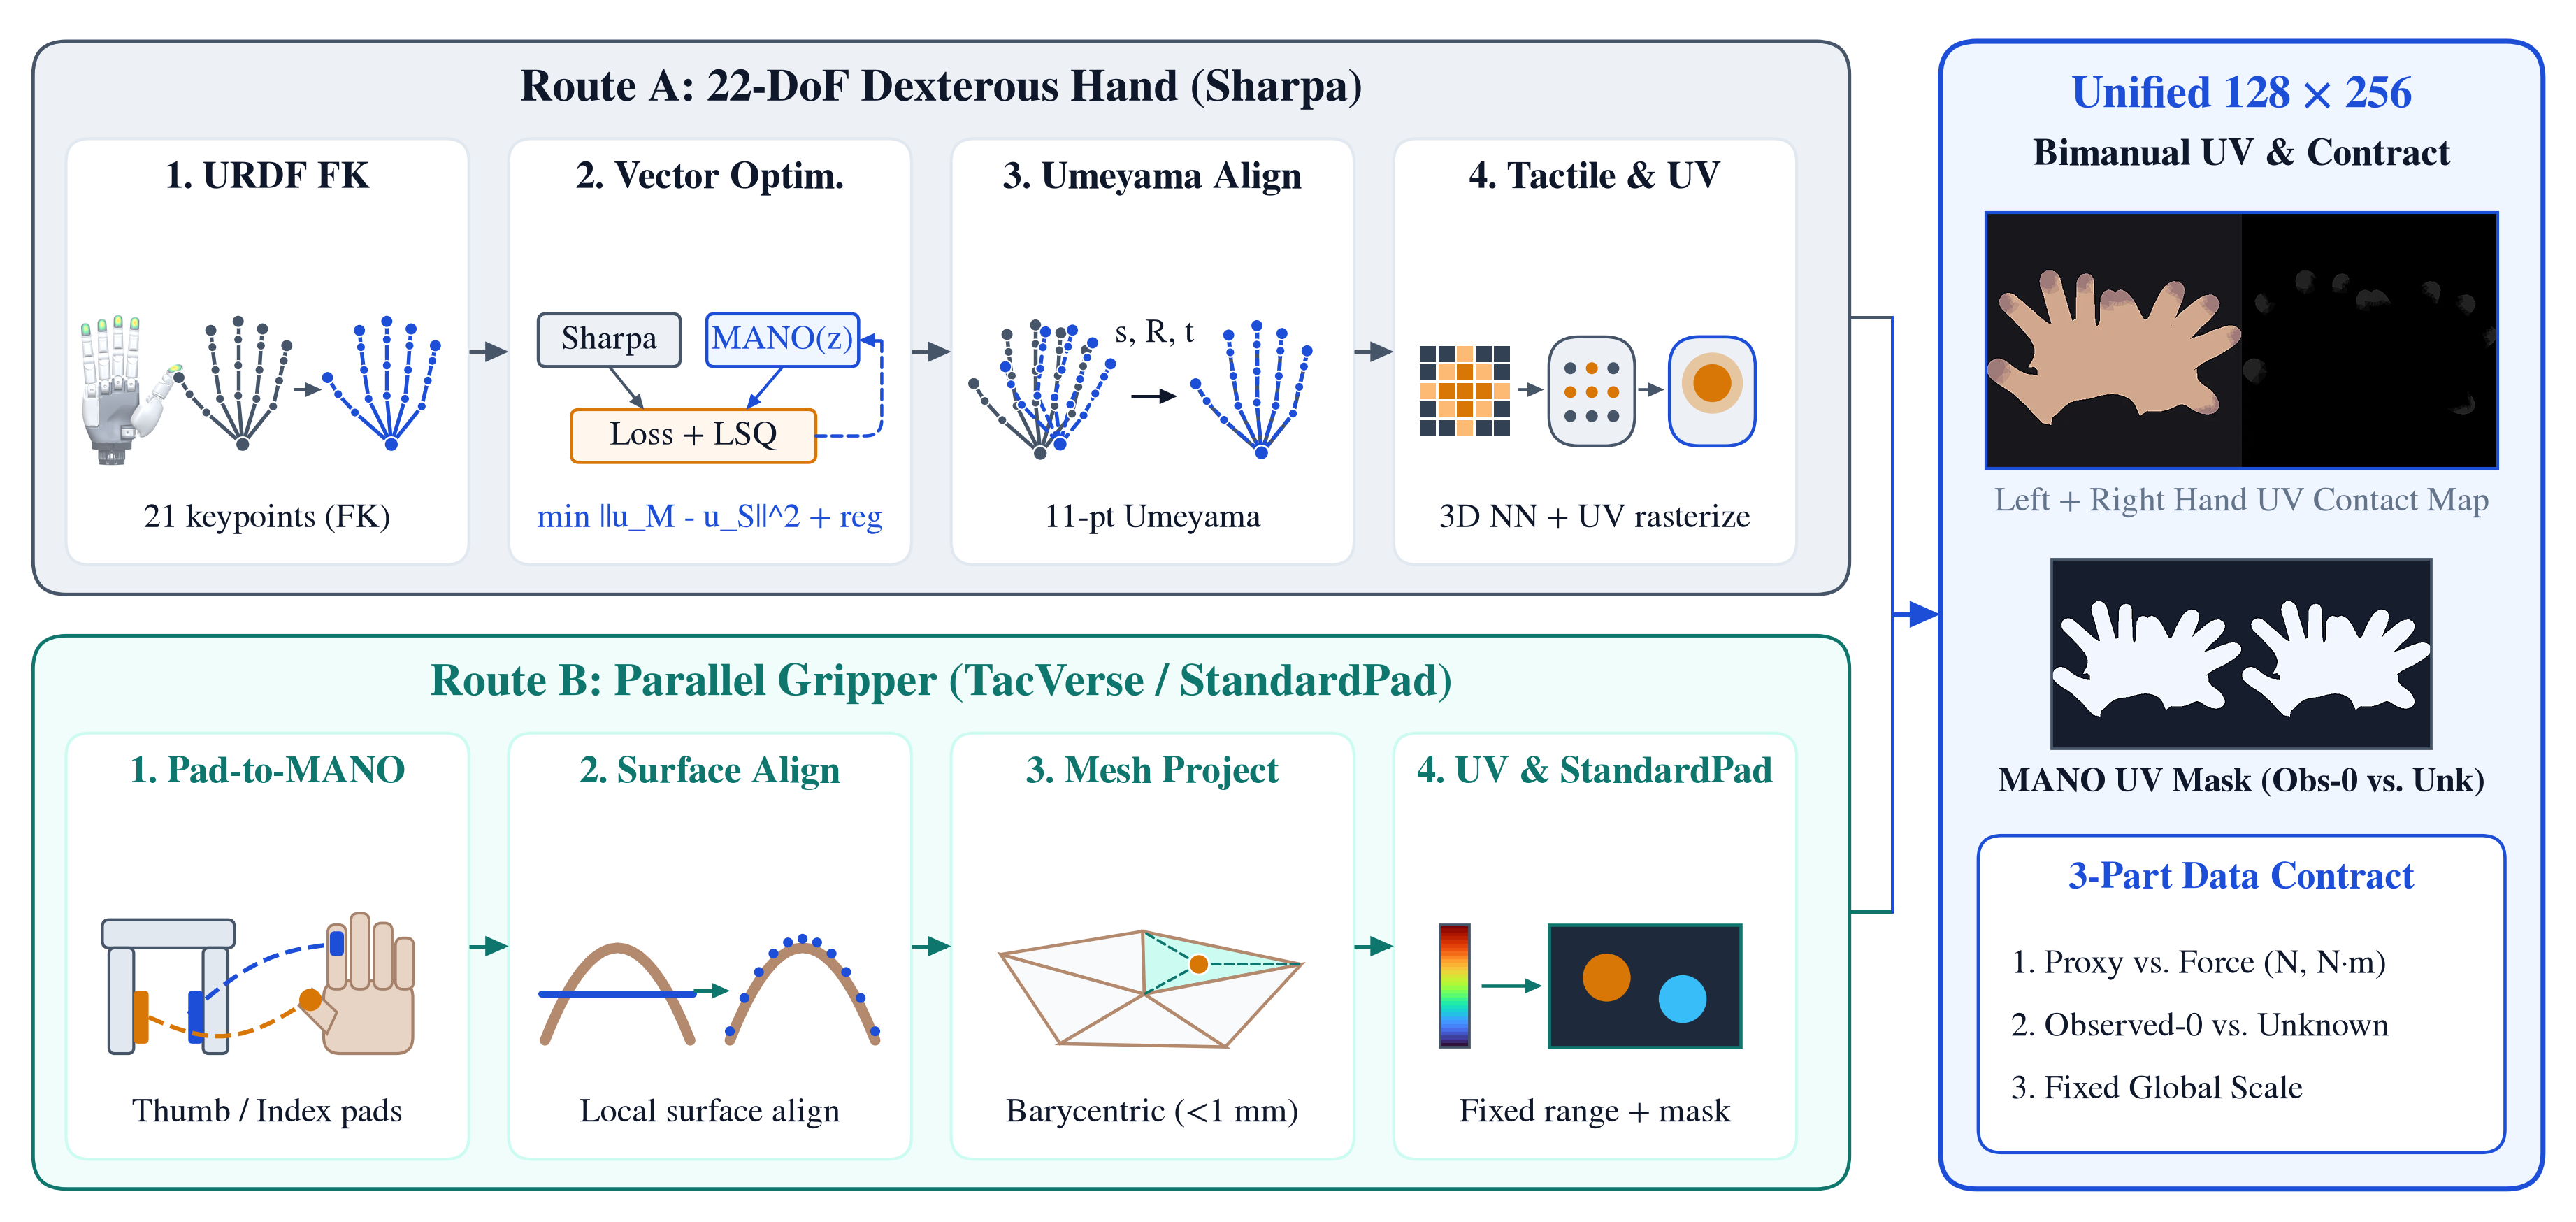
\includegraphics[width=0.95\textwidth]{img/fig2_retarget_pipeline_v2.png}
    \caption{Dual-route cross-embodiment retargeting under a unified four-stage structure. Both routes share the same macro-stages---(1)~Input \& Prep, (2)~MANO Alignment, (3)~Surface Projection, and (4)~Fixed-Scale UV Export---while adapting to embodiment geometry. \textbf{Route~A} maps 22-DoF Sharpa dexterous hands via URDF FK and luminance preprocessing, dynamic warm-started inverse bone-vector fitting with 11-anchor Umeyama seating, distal-phalanx local-frame cKDTree projection, and official UV rasterization with lookup-table recovery. \textbf{Route~B} maps parallel grippers via depth verification and flip-only alignment, static thumb/index pad assignment on a fixed 778-vertex MANO container, barycentric-to-UV texel averaging with \texttt{NaN}-preserving merge, and fixed-range proxy encoding with explicit validity masking (with \texttt{StandardPad} as a fallback for uncalibrated gripper corpora). Both routes converge into unified $128\times 256$ bimanual UV streams under our three-part data contract.}
    \label{fig:retarget_pipeline}
\end{figure*}

\paragraph{Route A: Articulated Dexterous Hands.}
For 22-DoF Sharpa dexterous hands equipped with fingertip deformation arrays, we perform dynamic per-frame kinematic retargeting (without neural training) followed by local-frame tactile projection:
\begin{enumerate}[leftmargin=*,nosep]
    \item \textbf{Input \& Prep (URDF FK \& Tactile Luma):} Because Sharpa's 22 joint angles and MANO's 45-DoF axis-angle rotations differ in joint count, axes, and link lengths, we evaluate the robot URDF via Pinocchio (writing joint states by joint name) to extract 21 MediaPipe-ordered, wrist-centered 3D keypoints $P^{\text{Sharpa}} \in \mathbb{R}^{21 \times 3}$ and 16 unit bone-direction targets $\{\hat{u}^{\text{Sharpa}}_k\}_{k=1}^{16}$. In parallel, observed fingertip tactile streams are converted to luminance and area-downsampled to $240\times 240$; missing finger channels are skipped without fabrication.
    \item \textbf{MANO Alignment (Dynamic Pose Fit \& Umeyama):} We optimize MANO global axis-angle rotation $r \in \mathbb{R}^3$ and 15-DoF PCA latent pose $z \in \mathbb{R}^{15}$ (using a flat-hand mean and $X$-axis mirroring for left hands) via regularized nonlinear least squares:
    \begin{equation}
        \min_{r, z} \sum_{k=1}^{16} \| \hat{u}^{\text{MANO}}_k(r, z) - \hat{u}^{\text{Sharpa}}_k(q) \|_2^2 + \lambda \|z\|_2^2,
    \end{equation}
    where $\lambda = 0.08^2$ and each frame is warm-started from the preceding solution $x_{t-1}$. Matching unit bone directions avoids bone-length mismatch artifacts. A closed-form Umeyama similarity transform $(s, R, t)$ \citep{umeyama1991least} fitted on 11 anchor keypoints (wrist, 5 finger roots, and 5 fingertips) then seats all 778 MANO vertices and 16 joints onto $P^{\text{Sharpa}}$.
    \item \textbf{Surface Projection (Distal-Frame cKDTree):} For each observed finger, we construct a finger-local orthonormal frame anchored at the distal fingertip and scaled by distal bone length, reducing sensitivity to global hand motion. MANO distal vertices (skinning weight $>0.2$) are queried against the manufacturer's $240\times 240\times 3$ sensor point cloud via a KD-tree ($j^* = \arg\min_j \|v^{\text{MANO}}_i - p^{\text{sensor}}_j\|_2$). Only vertices within a $6.5$~mm radius receive luminance values (closer fingers take precedence on overlap), scaled under a fixed saturation map $c = \mathrm{clip}(v/180, 0, 1)$.
    \item \textbf{Fixed-Scale UV Export (Official UV \& LUT):} Vertex intensities are averaged per triangular face (with reversed face winding for left hands) and rasterized onto the official $1024\times 1024$ MANO UV atlas using a cached, pose-invariant face-ID map with 1-pixel seam dilation. The atlas is nearest-neighbor downsampled to $128\times 128$ and inverted through a fixed lookup table back to canonical \texttt{uint8} contact-proxy maps alongside pose metadata and solver diagnostics.
\end{enumerate}

\paragraph{Route B: Two-Finger Parallel Grippers.}
Unlike articulated hands, two-finger parallel grippers lack human-like finger DoFs. Following the same four-stage structure, Route~B replaces dynamic pose fitting and 3D nearest-neighbor search with a static MANO container and direct barycentric texel projection:
\begin{enumerate}[leftmargin=*,nosep]
    \item \textbf{Input \& Prep (Depth Verification \& Flip Align):} Per-pad \texttt{float32} depth maps (reconstructed upstream from visuo-tactile RGB streams using temporally stable maximum-aperture no-contact reference windows) are verified against calibrated reference channels and optionally aligned via flip-only orientation transforms (\texttt{flip\_x}, \texttt{flip\_y}, or \texttt{rotate180}, without rescaling) when reusing left-hand calibrations.
    \item \textbf{MANO Alignment (Static 778-Vertex Container):} Rather than fitting per-frame hand poses, we treat the canonical 778-vertex MANO mesh as a \emph{fixed tactile container}, assigning the left gripper pad to the MANO thumb pad and the right pad to the MANO index pad while leaving the middle, ring, little fingers, and palm explicitly unobserved. Offline geometric calibration stores each valid sensor pixel's MANO face ID and barycentric weights $(b_0, b_1, b_2)$ ($\sum_i b_i = 1$) in a verified lookup table (\texttt{fixed\_mapping.h5}, $<1$~mm surface fit and $<10^{-8}$ vertex-reconstruction check).
    \item \textbf{Surface Projection (Barycentric UV \& \texttt{NaN} Merge):} Because each 3D mesh face shares identical barycentric weights with its 2D UV triangle ($P_{\text{UV}} = \sum_{i=0}^2 b_i\,\mathrm{UV}_i$), valid pixels are pre-mapped directly to $128\times 128$ official UV texel indices with zero per-frame 3D recomputation. Colliding finite depth samples within each finger are averaged per UV texel, and thumb and index rasters are merged with equal weight while preserving every unobserved texel strictly as \texttt{NaN} rather than zero-filling.
    \item \textbf{Fixed-Scale UV Export (Fixed Encode \& Valid Mask):} Finite texels are encoded as \texttt{uint8} contact proxies under a fixed global depth range $c = \mathrm{round}(255\cdot\mathrm{clip}((d - 0.001)/(0.4 - 0.001), 0, 1))$ (with optional \texttt{uint16} depth export over $[-0.001, 0.4]$, reserving $0$ for unknown), paired with an explicit binary observation validity mask (\texttt{valid.png}) separating observed-zero pads from uninstrumented regions.
\end{enumerate}

\paragraph{Extension to Uncalibrated Grippers (\texttt{StandardPad}).}
For parallel-gripper corpora lacking offline pixel-to-mesh geometric calibration, \bench{} provides a fallback \texttt{StandardPad} mode that projects rectangular taxel, depth, or pressure matrices onto the canonical thumb and index UV footprints using training-frozen per-texel median baselines and 99th-percentile scales (zero-centered for signed shear). This preserves spatial and temporal trend structure---onset, load evolution, contact migration, and inter-pad correlation---without assuming metric surface correspondence.

\subsection{Unified Six-Source Corpus and Audit}
\label{sec:dataset_stats}
Table~\ref{tab:dataset_stats} and Figure~\ref{fig:dataset_uv_examples} summarize the six manipulation corpora unified under \bench{}.
Five sources originate from Sharpa dexterous hands (deformation intensity proxies), including \texttt{FTP-1} with partial 3-finger coverage, while \texttt{TacVerse} contributes visuo-tactile parallel-gripper recordings (depth proxies) with explicit observation validity masks.
All unified streams undergo automated contract auditing for schema compliance, frame alignment, and validity-mask integrity, alongside per-frame solver diagnostics (Appendix~\ref{app:audit}).

\begin{figure*}[t]
    \centering
    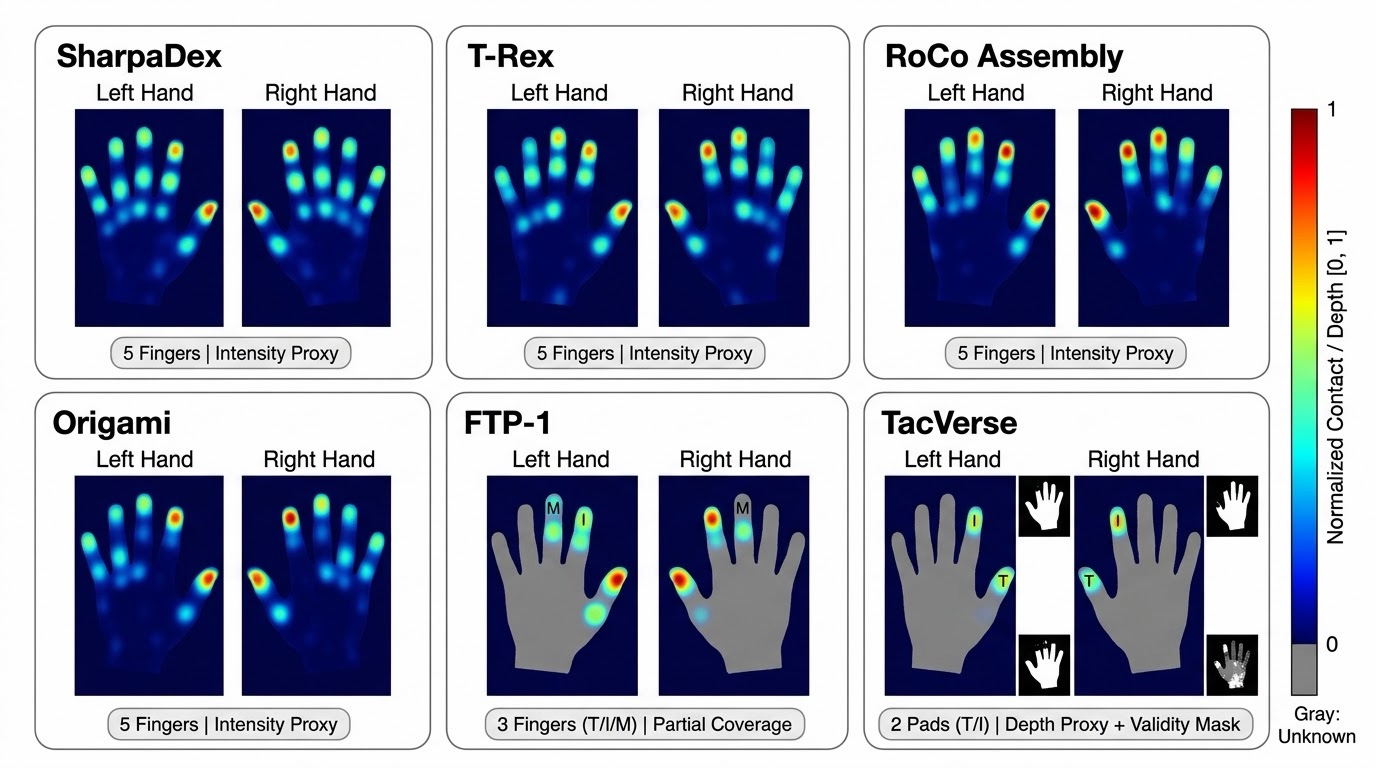
\includegraphics[width=0.95\textwidth]{img/fig3_dataset_uv_examples.jpg}
    \caption{Representative bimanual MANO UV examples across the six unified corpora. Five dexterous-hand sources (\texttt{SharpaDex}, \texttt{T-Rex}, \texttt{RoCo Assembly}, \texttt{Origami}, and partial 3-finger \texttt{FTP-1}) provide contact intensity proxies, while \texttt{TacVerse} provides parallel-gripper depth proxies with explicit validity masks separating observed-zero from unknown texels.}
    \label{fig:dataset_uv_examples}
\end{figure*}

\begin{table*}[t]
\centering
\small
\setlength{\tabcolsep}{5pt}
\begin{tabular}{llccccc}
\toprule
\textbf{Source Corpus} & \textbf{Embodiment} & \textbf{Signal Type} & \textbf{Coverage} & \textbf{Valid Mask} & \textbf{\# Episodes} & \textbf{\# Frames} \\
\midrule
SharpaDex & Dexterous Hand & Intensity proxy & 5 fingers & Planned & \tbd & \tbd \\
T-Rex & Dexterous Hand & Intensity proxy & 5 fingers & Planned & \tbd & \tbd \\
RoCo Assembly & Dexterous Hand & Intensity proxy & 5 fingers & Planned & \tbd & \tbd \\
Origami & Dexterous Hand & Intensity proxy & 5 fingers & Planned & \tbd & \tbd \\
FTP-1 & Dexterous Hand & Intensity proxy & 3 fingers (T/I/M) & Planned & \tbd & \tbd \\
TacVerse & Parallel Gripper & Depth proxy & 2 pads (T/I) & \checkmark & \tbd & \tbd \\
\midrule
\textbf{Total (Unified)} & \textbf{Dexterous + Gripper} & \textbf{2 Proxy Types} & \textbf{2--5 Fingers} & \textbf{Partial} & \tbd & \tbd \\
\bottomrule
\end{tabular}
\caption{Summary of the six tactile corpora unified into the canonical $128\times 256$ (30~FPS) MANO UV format. Raw corpus identifiers and audit details are listed in Appendix~\ref{app:audit}; exact episode and frame counts will be populated upon completion of the six-source manifest.}
\label{tab:dataset_stats}
\end{table*}

\section{The \bench{} Evaluation Suite}
\label{sec:benchmark}

\subsection{Hierarchical Probing Taxonomy (L0--L2)}
\label{sec:taxonomy}
\bench{} evaluates \emph{frozen} tactile encoder latents rather than comparing heterogeneous pre-training losses.
We organize evaluation into a three-tier hierarchy (summarized in Table~\ref{tab:task_matrix}):
\begin{itemize}[leftmargin=*,nosep]
    \item \textbf{L0 (Information Retention):} Verifies data contract compliance (\texttt{L0.0}), measures diagnostic native-decoder reconstruction (\texttt{L0.1}), and conducts primary cross-model comparison via a \emph{unified low-capacity probe decoder} (\texttt{L0.2}) reporting contact/non-contact MAE, Dice, IoU, total-load relative error, and peak error.
    \item \textbf{L1 (Frozen Readability):} Decouples readout into three sub-tiers:
    \texttt{L1a} \emph{Contact Proxies} (regional intensity proxy load, valid-region contact area, surface contact center, and multi-finger contact pattern);
    \texttt{L1b} \emph{Calibrated Physical Force/Wrench} (per-finger normal/tangential force $F_n, F_t$, 6-axis wrench, and common-frame resultant force---strictly gated on verified unit, coordinate, and time alignment); and
    \texttt{L1c} \emph{Temporal Contact Dynamics} (future $k$-frame proxy/force change $\Delta F$, contact onset/offset events, 5-stage contact phase, and Coulomb-verified slip).
    \item \textbf{L2 (Generalization and Robustness):} Evaluates frozen transfer under in-source OOD splits (\texttt{L2.in}), cross-source transfer (\texttt{L2.src}), cross-embodiment dexterous$\leftrightarrow$gripper transfer (\texttt{L2.emb}), cross-quantity transfer (\texttt{L2.qty}: zero-shot ranking/classification plus target-domain calibrated regression), and input perturbations (\texttt{L2.rob}: occlusion, additive noise, downsampling, and frame drop).
\end{itemize}

\begin{table*}[t]
\centering
\small
\setlength{\tabcolsep}{4.5pt}
\begin{tabular}{llll}
\toprule
\textbf{Tier} & \textbf{Sub-Task} & \textbf{Measurement Target} & \textbf{Primary Metrics} \\
\midrule
\multirow{3}{*}{\textbf{L0}} & L0.0 Contract Audit & Encoding, frame alignment, validity mask & Pass/Fail, bad-sample count \\
 & L0.1 Native Recon. & Frozen encoder + native latent-only decoder & Contact/Non-contact MAE, Dice, IoU \\
 & L0.2 Unified Recon. & Frozen encoder + shared small probe decoder & Contact/Non-contact MAE, Dice, IoU, Rel.\ Err. \\
\midrule
\multirow{4}{*}{\textbf{L1a}} & L1a.load & UV regional contact intensity proxy sum & $R^2$, Spearman $\rho$, NRMSE \\
 & L1a.area & Contact area ratio within valid region & MAE (percentage points) \\
 & L1a.center & Calibrated surface contact center (contact only) & Euclidean distance (mm) \\
 & L1a.pattern & Multi-finger binary contact combination & Macro-F1 \\
\midrule
\multirow{3}{*}{\textbf{L1b}} & L1b.force & Verified per-finger normal/tangential force & Per-finger $F_n, F_t$ MAE, RMSE (N) \\
 & L1b.wrench & Verified 6-DoF fingertip force \& torque & Per-axis MAE, RMSE (N / N$\cdot$m) \\
 & L1b.total & Common-frame whole-hand resultant force & Magnitude MAE (N) \\
\midrule
\multirow{4}{*}{\textbf{L1c}} & L1c.dF & Future $k$-frame force or proxy delta & NRMSE (proxy) / MAE in N (verified force) \\
 & L1c.event & Contact onset / offset detection & Event F1, latency (ms) \\
 & L1c.phase & 5-phase contact state (none/onset/load/unload/release) & Balanced Accuracy, Macro-F1 \\
 & L1c.slip & Incipient slip (verified shear/wrench sources only) & F1 \\
\midrule
\multirow{4}{*}{\textbf{L2}} & L2.in / L2.src & Held-out in-source / cross-source transfer & Zero-shot, calibrated, target upper bound \\
 & L2.emb & Dexterous hand $\leftrightarrow$ parallel gripper transfer & Ranking / classification + calibrated L1 \\
 & L2.qty & \texttt{sharpa\_intensity} $\leftrightarrow$ \texttt{depth\_proxy} & Zero-shot rank/cls + target-calibrated reg. \\
 & L2.rob & Occlusion, noise, downsampling, frame drop & Degradation curve vs.\ perturbation level \\
\bottomrule
\end{tabular}
\caption{Hierarchical evaluation taxonomy in \bench{}. L1b physical units (N, N$\cdot$m) are reported only when external wrench labels pass unit, coordinate, and temporal alignment verification. L3 (physics consistency) and L4 (closed-loop control) are reserved for future work.}
\label{tab:task_matrix}
\end{table*}

\subsection{Fair Frozen-Encoder Probing Protocol}
\label{sec:protocol}
All models are evaluated by extracting offline features from \emph{frozen} encoder checkpoints; pre-training is strictly decoupled from probing.
Within each task, every encoder shares identical inputs, labels, validity masks, and episode-level splits (default: 5\% validation sampled by whole episode with fixed seed 42; held-out test set read once).
To assess representation geometry beyond a single readout head, every L1/L2 task evaluates three standardized probes:
\begin{enumerate}[leftmargin=*,nosep]
    \item \textbf{Projected Readout:} $\text{Linear}(D, 256) \rightarrow \text{LayerNorm} \rightarrow \text{Linear}(256, C)$. Because LayerNorm introduces a nonlinearity, we term this a \emph{projected readout} rather than a strict linear probe, and explicitly report the input projection parameter count when latent dimension $D$ differs across encoders.
    \item \textbf{$k$-NN Probe:} Non-parametric $k$-nearest neighbors on pre-projection mean-pooled features, with $k$ selected solely on validation.
    \item \textbf{Attentive Readout:} 256-dim projection followed by single-query cross-attention and a linear head (with token count disclosed, as single-token attention cannot reflect spatial selection).
\end{enumerate}
For temporal tasks, standard clips use 16 frames at stride 1, whereas video-JEPA clips use 16 frames at stride 2; single-frame models consume only the last frame via an explicit adapter, and input budgets are always reported side by side.
By default, single-hand evaluation uses \emph{isolated} mode (masking the non-evaluated hand as unknown), while \emph{bimanual} context is evaluated in a separate explicit mode.
Every probe is trained with at least 3 random head seeds; we report episode-grouped bootstrap confidence intervals, paired permutation tests on identical test samples, valid/bad sample counts, and \texttt{null} for undefined metrics (e.g., contact MAE on non-contact frames is never zero-filled).

\subsection{Reference Tactile Encoder Suite}
\label{sec:encoders}
To validate \bench{} and provide strong baselines trained directly on our unified MANO UV corpus, we assemble four model groups:
\begin{itemize}[leftmargin=*,nosep]
    \item \textbf{Non-Learned \& Random Baselines:} Raw pixels (downsampled to $16\times 16$ per hand), train-fitted PCA (32-dim), and a fixed-seed random small CNN (64-dim).
    \item \textbf{\texttt{force\_encoder\_zero} (Pixel Reconstruction):} ConvNeXtV2-style CNN \citep{woo2023convnext} and ViT \citep{dosovitskiy2021image} encoders across four scales (\texttt{tiny}, \texttt{small}, \texttt{base}, \texttt{large}), trained on bimanual $128\times 256$ UV maps with a 512-dim global latent bottleneck.
    \item \textbf{\texttt{force\_encoder\_jepa} (Latent Prediction):} Four ViT scales $\times$ four recipes (\{\texttt{single\_frame}, \texttt{video}\} $\times$ \{\texttt{EMA}, \texttt{SIGReg}\}), outputting coverage-weighted backbone features (teacher backbone for EMA; online backbone for SIGReg, excluding the training projector).
    \item \textbf{External Candidate Adapters:} Via a generic TorchScript / adapter interface, \bench{} supports external tactile encoders (e.g., spatial vs.\ global branches of HY-X-Touch-fast, SharpaWave DeformEncoder, AnyTouch2, and Sparsh), strictly enforcing latent-only reconstruction (disclosing any input-contour bypasses) and pre-training data overlap audits.
\end{itemize}

\section{Experiments and Diagnostic Analysis}
\label{sec:experiments}

\subsection{Experimental Setup}
\label{sec:exp_setup}
All encoders are pre-trained on the unified MANO UV training split and frozen prior to offline feature extraction.
Unless stated otherwise, experiments follow the fair probing protocol in Section~\ref{sec:protocol}: episode-level splits (seed 42, 5\% validation, single-read held-out test), $\ge 3$ probe seeds, episode-grouped 95\% bootstrap confidence intervals, and paired permutation tests for model comparisons.
We explicitly separate single-frame (last-frame adapter) and multi-frame (16-frame stride-1 / stride-2) input budgets, as well as isolated single-hand vs.\ bimanual context modes.
\emph{Note: All tables below define the formal experimental protocol and reporting schema; entries marked \tbd{} will be populated upon completion of full six-source pre-training and independent test evaluation.}

\subsection{Information Retention and Frozen Readability (L0 \& L1)}
\label{sec:exp_l0_l1}
Table~\ref{tab:l0_retention} evaluates L0.2 unified small-decoder reconstruction to measure how faithfully each frozen latent preserves spatial contact geometry and intensity trends, decoupled from native decoder capacity.
Table~\ref{tab:l1_readability} reports L1a contact proxy readability (\texttt{load}, \texttt{area}, \texttt{center}, \texttt{pattern}) and L1c temporal dynamics (\texttt{dF}, \texttt{event}, \texttt{phase}) across projected readout, $k$-NN, and attentive probes.
Where external force/wrench labels pass unit, coordinate, and temporal alignment verification, L1b calibrated physical force results will be reported separately in Newtons (N / N$\cdot$m).

\begin{table*}[t]
\centering
\small
\setlength{\tabcolsep}{4.5pt}
\begin{tabular}{llcccccccc}
\toprule
\textbf{Model Family} & \textbf{Spec / Recipe} & \textbf{Latent} & \textbf{Input} & \textbf{Contact} & \textbf{Non-Cont.} & \textbf{IoU} & \textbf{Dice} & \textbf{Load Rel.} & \textbf{Peak} \\
 &  & \textbf{Dim} & \textbf{Mode} & \textbf{MAE $\downarrow$} & \textbf{MAE $\downarrow$} & \textbf{$\uparrow$} & \textbf{$\uparrow$} & \textbf{Err. $\downarrow$} & \textbf{Err. $\downarrow$} \\
\midrule
Raw Pixels & $16\times 16$ downsample & 256 & 1f-iso & \tbd & \tbd & \tbd & \tbd & \tbd & \tbd \\
PCA & Train-fit linear & 32 & 1f-iso & \tbd & \tbd & \tbd & \tbd & \tbd & \tbd \\
Random CNN & Fixed-seed init & 64 & 1f-iso & \tbd & \tbd & \tbd & \tbd & \tbd & \tbd \\
\midrule
\texttt{zero} CNN & tiny / small / base / large & 512 & 1f-iso & \tbd & \tbd & \tbd & \tbd & \tbd & \tbd \\
\texttt{zero} ViT & tiny / small / base / large & 512 & 1f-iso & \tbd & \tbd & \tbd & \tbd & \tbd & \tbd \\
\texttt{JEPA} ViT & 1f-EMA / 1f-SIGReg & $D_{\text{vit}}$ & 1f-iso & \tbd & \tbd & \tbd & \tbd & \tbd & \tbd \\
\texttt{JEPA} ViT & vid-EMA / vid-SIGReg & $D_{\text{vit}}$ & 16f-s2 & \tbd & \tbd & \tbd & \tbd & \tbd & \tbd \\
\midrule
External (TBD) & HY-X / SharpaWave / etc. & \tbd & \tbd & \tbd & \tbd & \tbd & \tbd & \tbd & \tbd \\
\bottomrule
\end{tabular}
\caption{L0.2 Unified Small-Decoder Reconstruction results on the held-out test set. All models share an identical low-capacity probe decoder to measure latent information retention fairly.}
\label{tab:l0_retention}
\end{table*}

\begin{table*}[t]
\centering
\small
\setlength{\tabcolsep}{4pt}
\begin{tabular}{llcccccccc}
\toprule
\textbf{Encoder} & \textbf{Probe} & \multicolumn{4}{c}{\textbf{L1a: Contact Proxy Readability}} & \multicolumn{3}{c}{\textbf{L1c: Temporal Dynamics}} & \textbf{L1b} \\
\cmidrule(lr){3-6} \cmidrule(lr){7-9} \cmidrule(lr){10-10}
 &  & \textbf{Load} ($R^2\uparrow$) & \textbf{Area} (MAE$\downarrow$) & \textbf{Center} (mm$\downarrow$) & \textbf{Pattern} (F1$\uparrow$) & \textbf{$\Delta F$} (NRMSE$\downarrow$) & \textbf{Event} (F1$\uparrow$) & \textbf{Phase} (Bal.\ Acc$\uparrow$) & \textbf{$F_n/F_t$} (N$\downarrow$) \\
\midrule
Raw / PCA / Rand. & Proj / kNN & \tbd & \tbd & \tbd & \tbd & \tbd & \tbd & \tbd & \tbd \\
\texttt{zero} CNN & Proj / kNN / Attn & \tbd & \tbd & \tbd & \tbd & \tbd & \tbd & \tbd & \tbd \\
\texttt{zero} ViT & Proj / kNN / Attn & \tbd & \tbd & \tbd & \tbd & \tbd & \tbd & \tbd & \tbd \\
\texttt{JEPA} (1f) & Proj / kNN / Attn & \tbd & \tbd & \tbd & \tbd & \tbd & \tbd & \tbd & \tbd \\
\texttt{JEPA} (video) & Proj / kNN / Attn & \tbd & \tbd & \tbd & \tbd & \tbd & \tbd & \tbd & \tbd \\
\bottomrule
\end{tabular}
\caption{L1 Frozen Readability results across projected readout (Proj), $k$-NN, and attentive (Attn) probes. L1a evaluates UV contact proxy trends; L1b physical force (N) is reported only on externally verified wrench subsets.}
\label{tab:l1_readability}
\end{table*}

\subsection{Cross-Source, Cross-Embodiment, and Perturbation Generalization (L2)}
\label{sec:exp_l2}
Table~\ref{tab:l2_generalization} summarizes generalization across three transfer axes:
(1) \emph{Cross-source (\texttt{L2.src})} among the five Sharpa dexterous-hand datasets;
(2) \emph{Cross-embodiment and cross-quantity (\texttt{L2.emb} / \texttt{L2.qty})} between Sharpa dexterous hands (\texttt{sharpa\_intensity}) and TacVerse parallel grippers (\texttt{depth\_proxy}), reporting zero-shot ranking/classification, few-shot target-domain calibrated regression, and target-domain upper bounds; and
(3) \emph{Perturbation robustness (\texttt{L2.rob})} under controlled occlusion, Gaussian noise, spatial downsampling, and frame dropout (with labels anchored to unperturbed inputs).
Pre-training source overlap with target domains is explicitly disclosed for every transfer pair.

\begin{table*}[t]
\centering
\small
\resizebox{\textwidth}{!}{%
\begin{tabular}{lccccccc}
\toprule
\textbf{Encoder} & \multicolumn{2}{c}{\textbf{L2.src (Sharpa Cross-Src)}} & \multicolumn{3}{c}{\textbf{L2.emb / L2.qty (Dexterous $\leftrightarrow$ Gripper)}} & \multicolumn{2}{c}{\textbf{L2.rob (Perturbations)}} \\
\cmidrule(lr){2-3} \cmidrule(lr){4-6} \cmidrule(lr){7-8}
 & \textbf{Zero-Shot} & \textbf{Calibrated} & \textbf{Zero-Shot} ($\rho$/F1) & \textbf{Calibrated} & \textbf{Target UB} & \textbf{Occ./Noise} & \textbf{Down./Drop} \\
\midrule
Raw / PCA / Rand. & \tbd & \tbd & \tbd & \tbd & \tbd & \tbd & \tbd \\
\texttt{zero} CNN & \tbd & \tbd & \tbd & \tbd & \tbd & \tbd & \tbd \\
\texttt{zero} ViT & \tbd & \tbd & \tbd & \tbd & \tbd & \tbd & \tbd \\
\texttt{JEPA} (1f / video) & \tbd & \tbd & \tbd & \tbd & \tbd & \tbd & \tbd \\
\bottomrule
\end{tabular}%
}
\caption{L2 Generalization and Robustness protocol. For cross-quantity transfers (\texttt{sharpa\_intensity} $\leftrightarrow$ \texttt{depth\_proxy}), zero-shot evaluation uses rank/classification metrics rather than uncalibrated gray-level errors.}
\label{tab:l2_generalization}
\end{table*}

\subsection{Controlled Ablations and Diagnostic Findings}
\label{sec:exp_ablations}
To isolate architectural and training-objective effects under controlled data budgets, we organize six diagnostic comparisons (Table~\ref{tab:ablations}):
(1) \textbf{Architecture (CNN vs.\ ViT):} Comparing \texttt{zero} CNN and ViT across \texttt{tiny}--\texttt{large} while reporting parameter count, latent dimensionality, and inference cost.
(2) \textbf{Objective (Reconstruction vs.\ Latent Prediction):} Comparing pixel-reconstruction (\texttt{zero}) against latent prediction (\texttt{JEPA} EMA and SIGReg).
(3) \textbf{Spatial vs.\ Global Latents:} Comparing compact 512-dim global bottlenecks against multi-token spatial latents while explicitly disclosing total latent element counts.
(4) \textbf{Temporal Context (Single-Frame vs.\ Video):} Quantifying the gain of 16-frame video encoders over single-frame encoders on L1c future-change and event tasks.
(5) \textbf{Hand Context (Isolated vs.\ Bimanual):} Measuring the benefit of bimanual context versus isolated single-hand inputs.
(6) \textbf{Scaling and Stability:} Separating training stability (convergence rate, numerical precision) from downstream probing gains across model scales and data fractions (1\% / 10\% / 100\%).

\begin{table}[t]
\centering
\small
\resizebox{\columnwidth}{!}{%
\begin{tabular}{llcc}
\toprule
\textbf{Diagnostic Axis} & \textbf{Controlled Variants} & \textbf{L0.2} & \textbf{L1 / L1c} \\
\midrule
Architecture & \texttt{zero} CNN vs.\ ViT & \tbd & \tbd \\
Objective & \texttt{zero} vs.\ JEPA (EMA/SIGReg) & \tbd & \tbd \\
Latent Form & Global (512d) vs.\ Spatial tokens & \tbd & \tbd \\
Temporal & Single-frame vs.\ 16f Video & \tbd & \tbd \\
Hand Context & Isolated vs.\ Bimanual & \tbd & \tbd \\
Model Scale & \texttt{tiny} / \texttt{small} / \texttt{base} / \texttt{large} & \tbd & \tbd \\
\bottomrule
\end{tabular}%
}
\caption{Summary of controlled ablation axes in \bench{}.}
\label{tab:ablations}
\end{table}

\section{Conclusion}
\label{sec:conclusion}

We introduced \bench{}, an end-to-end cross-embodiment tactile retargeting pipeline, unified canonical dataset, and frozen representation benchmark.
By mapping both articulated dexterous hands and two-finger parallel grippers onto a shared $128\times 128$ MANO UV atlas under a strict fixed-scale data contract, \bench{} enables apples-to-apples evaluation of frozen tactile encoders across information retention (L0), contact proxy, verified physical force, and temporal dynamic readability (L1), and cross-domain generalization (L2).
Together with our controlled suite of reconstruction (\texttt{zero}) and latent-prediction (\texttt{JEPA}) tactile encoders, \bench{} provides a reproducible foundation for studying what tactile representations capture and how well they transfer across robot embodiments.

\section*{Limitations}
\label{sec:limitations}

We highlight several important technical boundaries and limitations of the current framework:
\begin{itemize}[leftmargin=*,nosep]
    \item \textbf{Contact Proxy vs.\ Calibrated Physical Force:} UV grayscale values represent fixed-scale tactile intensity (Sharpa) or depth proxy trends (TacVerse), not calibrated Newton forces. Cross-source gray levels are not directly comparable in absolute physical units, and L1b physical force/wrench reporting requires independent external labels verified for units, coordinate frames, and temporal alignment.
    \item \textbf{Route~A Retargeting Accuracy and Coverage Masks:} Inverse vector retargeting on Sharpa hands exhibits non-zero fingertip alignment residuals (e.g., 22.96~mm left / 41.97~mm right RMS on \texttt{SharpaDex} ep20), and frames hitting the 40-evaluation cap are retained with \texttt{solver\_success=False}; exported poses should therefore be filtered by residual before serving as kinematic ground truth. Furthermore, current Sharpa UV outputs lack an explicit per-source validity mask, meaning zero values can conflate observed-zero contact with uncovered surface regions (e.g., 3-finger coverage in \texttt{FTP-1-sharpa}).
    \item \textbf{Route~B Reference Candidates and Right-Hand Mapping:} Automated TacVerse no-contact reference frames are static maximum-aperture \emph{candidates} rather than guaranteed zero-contact ground truth. Additionally, right-hand TacVerse UV maps currently reuse the left-hand surface correspondence (\texttt{unvalidated-mapping}, diagnostic only), and the offline adaptive-morphology fitting procedure generating \texttt{fixed\_mapping.h5} requires full documentation and standalone release.
    \item \textbf{Scope of Evaluation and Preliminary Status:} Physics consistency (L3) and closed-loop manipulation control (L4) remain future work. Dedicated event-latency matching and full six-source independent test evaluations are ongoing and will replace the placeholder entries in Section~\ref{sec:experiments}.
\end{itemize}

\section*{Ethics Statement}
All tactile datasets unified in this work are derived from publicly available or institutionally authorized robotic manipulation corpora containing no personally identifiable human subject data.
Our retargeting and benchmarking software introduces no direct dual-use safety hazards; however, deploying uncalibrated tactile proxies in safety-critical physical human-robot interaction without hardware-level force calibration could cause unintended contact forces, which we explicitly caution against in our data contract and limitations.


\bibliography{references}

\appendix
\section{Retargeting Implementation Details}
\label{app:retarget}
\paragraph{Sharpa Route (Route~A).}
Joint states follow the 22-DoF URDF ordering per hand. Tactile mosaics ($2\times 5$) are converted to luminance and downsampled via \texttt{INTER\_AREA} to $240\times 240$ per finger, synchronized to state timestamps via millisecond seeking.
The 16 inverse vector-retargeting residuals yield a 48-dim unit-vector residual concatenated with $0.08\theta \in \mathbb{R}^{15}$.
A GPU-batched finite-difference Jacobian variant skins only the 5 fingertip vertices during optimization and reproduces CPU outputs identically.

\paragraph{TacVerse and \texttt{StandardPad} Routes (Route~B).}
TacVerse $400\times 700$ frames are transposed to $700\times 400$ for Xense SDK 2.1.2 depth inference without cropping or color distortion, then transposed back.
Optional \texttt{uint16} depth encoding maps $[-0.001, 0.4]$ to $[1, 65535]$ with 0 reserved for unknown (raising an error on out-of-range values rather than silent clipping).

\section{Probing and Statistical Testing Details}
\label{app:probes}
Probe hyperparameters (learning rate, epochs, $k$ for $k$-NN) are selected exclusively on the 5\% episode-level validation split (seed 42).
Formal benchmark runs use at least 3 probe seeds and episode-grouped bootstrap resampling to compute 95\% confidence intervals, alongside paired permutation tests on identical evaluation samples.
All reports record valid sample counts, bad sample counts, and explicit \texttt{null} entries for undefined metrics.


\end{document}
